% IN THIS SECTION SHOW SOME OF OUR TRANSLATED CODE... AND WALK THROUGH IT THE SAME WAY YOU DID WITH THE CONCEPT IN RESOLVE. BUT BEFORE YOU DO THAT, SHOW THE PICTURE (The one thats already here showing high level relationships and update it!).
\section{Implementation}
Development of our C translation tool can be logically partitioned into three distinct pieces: 
\begin{enumerate}
\item Arriving at a translation model (or, strategy) for an efficient, reliable C representation of RESOLVE.
\item Implementing reusable mechanisms for carrying out the C code generation process.
\item Creation of a memory manager capable of safely allocating and freeing dynamic memory required by the generated code.
\end{enumerate}
In this section we discuss each of these phases using the LED component developed in Section \ref{sec:specifiying}.

\subsection{C Translation Model}
One of the primary challenges in translating from RESOLVE to C is finding a suitable C analog for each RESOLVE module and the constructs allowable in each. Indeed, since we are dealing with an environment where functional correctness is a primary concern, it is important that the code generated by our tool represents as closely as possible the original RESOLVE source. In an effort to make such considerations, at the highest level, the C code generated makes special considerations for facilities, concepts, and realizations. 

The memory model must also be considered as an additional verifiable component. Currently, RESOLVE is not capable of creating a complete specification of memory\footnote{RESOLVE is an object based language and has variable sized structures. Using dynamically allocatable memory is the favored approach to allow arbitrarily sized data.}. Thus, a memory model must be realized without a specification. To provide a straight forward translation from RESOLVE to C, we provide a dynamically-based memory allocator for use on embedded systems.

The relationship between the RESOLVE module type and c code generated is depicted at a high level in Figure \#. Unsurprisingly, concepts are represented in C by a single header \texttt{.h}. Some realizations connected to concepts are \texttt{externally} realized, denoting that they are not generated from RESOLVE. Additionally concepts can be \texttt{enhanced by} adding new enhancement components to the concept. RESOLVE facilities then produce corresponding \texttt{.h/c} files that provides the application interface implementation of concepts.

%Unsurprisingly, concepts are represented in C by a single header .h listing the various methods 

\subsection{Translator Implementation}

\subsubsection{AST Traversal}
Translation is performed over the course of a traversal of RESOLVE's abstract syntax tree (AST). The traversal mechanism used is a dervivative of the visitor pattern that provides a SAX-dom style pre-post traversal over all nodes in the tree. Thus, for any given node present, a total of two visits occur: One corresponding to the node being `hit' during the pre traversal stage, and one for the post. 

To make this more concrete, consider the following dummy operation.

\begin{verbatim}
Operation Nothing(); Procedure
        Var X : Integer;
        X := 3;
end Nothing;
\end{verbatim}

Shown in Figure \ref{fig:ast} is the AST representation of operation \texttt{Nothing}. Here, language constructs are represented as labeled boxes, while the actual traversal over these constructs -- and the order in which it is performed -- is communicated on the right via the call stack. Each of these calls are received in the translator in the order in which they are visited within the tree. It is up to the client (in this case, the author of the C-translator) to decide which of these methods they wish to override and perform custom actions within. 

We feel this particular traversal pattern lends itself to task of source to source translation for the following reasons:

\begin{itemize}
\item A visit method for a construct provides a convenient encapsulation of all the logic required to translate RESOLVE construct $x$ to appropriate C construct $y$.

\item Overriden visit methods apply to every instance of a construct -- meaning RESOLVE's C translator requires few (if any) loops, as the walk itself serves as the method of iteration.

\item Finally, only the visit methods for the constructs we currently wish to process need to be overridden. This makes it easy to tweak and optimize the size of the translator's codebase, implementing only visit method for language constructs that explicitly require translation.  
\end{itemize}

\subsubsection{Translation output}
Output of translated code is done using \textit{Stringtemplate} -- a third-party tool written in Java that allows users to define parameterizable templates. Like the name suggests, a template is simply ``a document with holes" that the user choses when and how to fill. 

An example C function definition template is shown below.

\begin{verbatim}
function_def(modifier, type, name, params, 
                               vars, stmts) ::= <<
<modifier> <type> <name> (<params; sep = ", ">) {
    <vars; sep = "\n">
    <stmts; sep = "\n">
}>>
\end{verbatim}

User supplied attributes, enclosed in \texttt{<..>}, indicates the position of that attribute relative to others. It is entirely up to the user to define which attributes to fill in, and how complex they want them to be. For example, the user might choose to fill the \texttt{params} attribute with a simple string, or a separately defined \texttt{parameter} template, which in turn might use another separately defined \texttt{type} template.

\begin{verbatim}
parameter(type, name) ::= "<type> <name>"
\end{verbatim}

In the context of language translation, these templates, when stored on a stack and manipulated over the course of the aforementioned AST traversal, help simplify the task of producing complicated, structured blocks of C output. For instance, upon visiting \texttt{preOperationDec}, a \texttt{function\_def} template can be instantiated by the client and pushed onto a global translation stack with its \texttt{name}, return \texttt{type}, and \texttt{modifier} attributes filled in. As \texttt{preOperationDec}'s children are visited, the \texttt{function\_def} template currently at the top of the stack receives similarly constructed parameter, variable, and statement templates from the nodes being walked. Upon reaching \texttt{postOperationDec}, we can be assured that the function has been completely filled in with the appropriate templates -- assuming the user has implemented the children's visit methods.

Hence, the only actual work being performed within visit methods is forwarding appropriate information from tree-node it represents, to an externally defined template. This allows us to exploit (in shameless design pattern parlance) a strict model view controller (MVC) separation in the translator's codebase between the mechanism that does the AST visiting (controller), the tree nodes from which we're adding information to templates (model), and the external file containing all available C language templates (view).

%One of the primary allures of this approach to translation is that that adheres to strict MVC design principles -- meaning that all output logic is distinctly separated from translation related logic. 

%We take advantage of these pre post methods using templates and simple stack to implement 


%Going even further, we demonstrate this by showing the steps taken to translate a simple operation declaration \texttt{nothing} to C.

% for each construct to remain encapsulated within that method, and (almost) completely eliminates the need for complex loop or iteration mechanisms. 


%This particular traversal pattern lends itself well to the language translation challenge (specifically source to source) where the pre methods align naturally with beginning of a construct, and conclude with its corresponding post method.  For instance, in the case above, this allows us, upon receiving a callback for In an effort to keep logic implementing our translator distinct and separate from the output language, we used a model view controller framework for implementing 

%To illustrate this, consider once again facility \texttt{DoNothing}.

\subsection{Memory Allocation}

Dynamic memory allocation does not lend itself well with an embedded programming paradigm. With hardware constraints, embedded systems have limited capacities on RAM. The telos motes are limited to 128 bytes of RAM. Many programs, however, require dynamic memory allocation to be used, including RESOLVE, in order to make it extensible. Previous RESOVE translations to C required static memory allocation \cite{regula:2010}. In this section a stack based dynamic memory allocator is introduced.

\subsubsection{Allocation using \texttt{salloc}}

The \texttt{salloc()} is a first fit memory allocator. Rather than allocating on the heap, \texttt{salloc()} uses the stack. At compilation, the allocator provisions a fixed size of memory. It requires a small section of meta-data called a block which contains information of about the size of memory allocated, neighboring blocks, as well if the block is free or not. A sample representation of the stack shown in figure \ref{fig:stack}, is a typical example of allocated memory on the stack.

\begin{figure}[!htb]
\centering
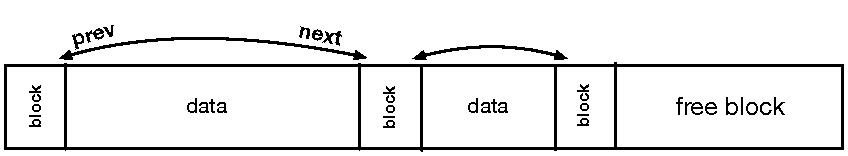
\includegraphics[scale=.55]{figs/stack.pdf}
\caption{Representation of memory stack}
\end{figure}
\label{fig:stack}

\subsubsection{Deallocation using \texttt{sfree}}

A memory allocator must provide a mechanism to release, or free memory in order to indicate that it is not being used and can be reallocated for something else. The \texttt{sfree()} operation is an analogous implementation to the standard C \texttt{free()} function for the stack.

\begin{figure}[!htb]
\centering
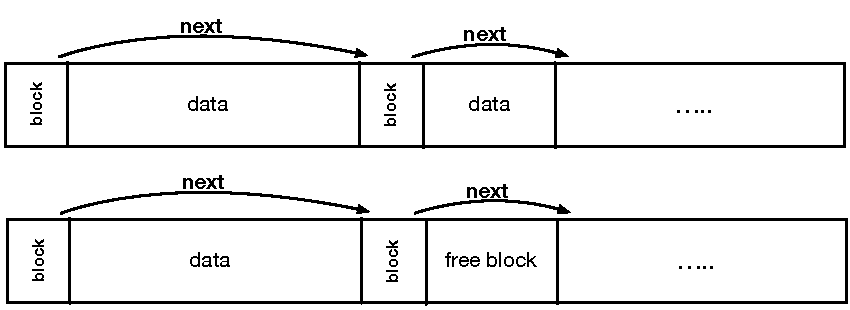
\includegraphics[scale=.55]{figs/sfree.pdf}
\caption{sfree to free memory}
\end{figure}
\label{fig:free}
 
\subsubsection{Optimizations}

A common problem that can occur in memory allocation is fragmentation.  As shown in figure \ref{fig:fragmentation}, fragmentation can lead to inefficient and increased memory usage. This problem is magnified on embedded systems with limited memory capabilities. Simple optimizations can be made however to reduce fragmentation. Splitting is one optimization that \texttt{salloc()} to maximize memory usage. Shown in figure \ref{fig:split}, blocks can be split to the size that is required. Another means of optimizing memory usage is joining together freed blocks. When a call to \texttt{sfree()} is made, neighboring blocks are coalesced together, as shown in figure \ref{fig:fuse}.

\begin{figure}[!htb]
\centering
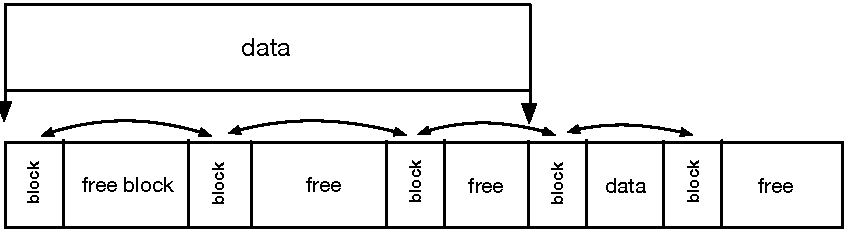
\includegraphics[scale=.55]{figs/fragmentation.pdf}
\caption{fragmentation}
\end{figure}
\label{fig:fragmentation}

\begin{figure}[!htb]
\centering
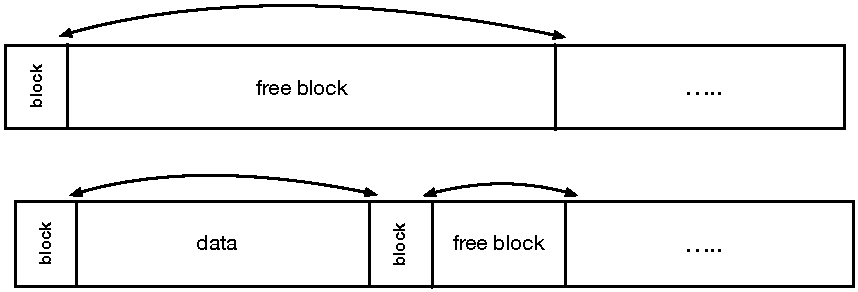
\includegraphics[scale=.55]{figs/split.pdf}
\caption{block splitting}
\end{figure}
\label{fig:split}

\begin{figure}[!htb]
\centering
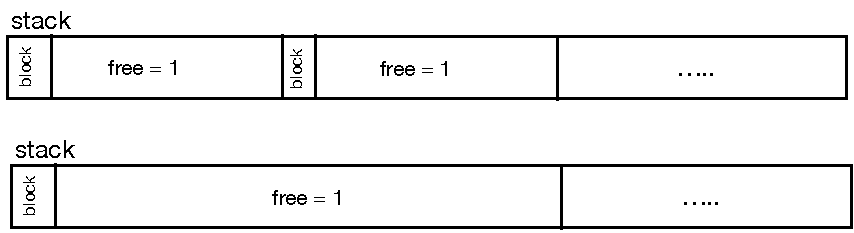
\includegraphics[scale=.55]{figs/fuse.pdf}
\caption{block fusing}
\end{figure}
\label{fig:fuse}
%A stack-based approached to dynamic memory allocation requires a fixed size of memory to be set prior to compilation. 
%To date there have been very few practical applications of verifiable code on physical media. 

\subsection{An LED Implementation}

\begin{verbatim}
void LED_Telos_create() {
		Std_Boolean_Fac_create();
		Std_Integer_Fac_create();
		Std_Clock_Fac_create();
		r_type_ptr __arg_0 = Std_Integer_Fac_Var.core->createFromInteger(4, Std_Integer_Fac_Var.core->Integer);
		LED_Telos_Facility_Var.core = new_Std_LED_Realiz_for_Leds_Template(__arg_0);
		LED_Telos_Facility_Var.Toggling_Capability = new_Toggling_Capability_of_Leds_Template(LED_Telos_Facility_Var.core);
		Std_Integer_Fac_Var.core->Integer->destroy(__arg_0, Std_Integer_Fac_Var.core->Integer);
}
\end{verbatim}